\chapter{Connectedness}

\section{Definitions}
    \subsection{Walk}
        For 2 vertices $v$ and $w$, a \textbf{walk} from $v$ to $w$ is an alternating sequence $v_0 e_1 v_a e_1 \cdots e_n v_n$ of vertices $v_0, \cdots, v_n$ and edges $e_1, \cdots, e_n$. such  that the sets of ends of $e_i$ is {$v_{i-1} , v_i$} and $v_0 =v, v_n=w, n \geq 0$
    \subsection{Trail}
        A \textbf{trail} is a walk without using the same edge twice
    \subsection{Path}
        A \textbf{path} is a walk not using any vertex twice
    \subsection{Closed trail}
        A walk from $v$ to $w$ is \textbf{closed} if $v=w$
        A \textbf{circuit} is also a closed trail
    \subsection{Cycle}
        A \textbf{cycle} is a circuit $v_0 e_1 v_a e_1 \cdots e_n v_n$ such that $v_0, v_1, \cdots, v_{n-1}$ are distinct\\
        $Circuit\Rightarrow cycle$\\
        $Circuit\not\Leftarrow cycle$
\section{Theorems}
    \subsection{Lemma}
        \subsubsection{Definition}
             If $G$ has a walk from $x$ to $y$, then $G$ has a path from $x$ to $y$
        \subsubsection{Proof}
            \textbf{Induction on n}\\
            Let's call n the length of the walk $W$ from $x$ to $y$

            \begin{enumerate}
                \item If $n = 0$ : trival
                \item If $n \neq 0$ :
                    We may assume $W$ is not a path (Else, trivial)\\
                    $W$ has a vertex $z$ that is visited more that once.\\
                    $\begin{array}{c}
                        x=v_0 e_1 v_1 e_2 \cdots z \cdots z \cdots e_n y \\
                        \Downarrow\\
                        W'=v_0 e_1 v_1 e_2 \cdots z \cdots e_n y
                    \end{array}$\\
                    $W'$ is a walk from $x$ to $y$ whose length is $<$ $n$\\
                    By the induction hypothesis, $G$ has a path from $x$ to $y$\\
                    $G$ is connected $\Leftrightarrow \forall x, y \in V(G), G$ has a path from $x$ to $y$
            \end{enumerate}
            

    \subsection{$\sim$ relation}
        \subsubsection{Definition}
            $\forall x,y \in V(G), x \sim y \Leftrightarrow G$ has a path from $x$ to $y$
        \subsubsection{Equivalent ?}
        \[ \left \{
            \begin{array}{l}
                \textbf{symmetric}: x\sim y \Rightarrow  y\sim x\\
                \textbf{reflexive}: x\sim x\\
                \textbf{transitive}: x\sim y, y\sim z \Rightarrow x\sim z
            \end{array}
        \right .\]
    \subsection{Connected component graph}
        A \textbf{connected component} of a graph $G$ is a subgraph induced on an equivalence class of $(V(G), \sim)$\\
        i.e. : a component is a maximal connected subgraph
        \begin{itemize}
            \item If $C, D$ are component, then $C=D$ or $V(C) \cap V(D) = \emptyset$
            \item $G$ is disconnected $\Leftrightarrow V(G)$ can be partitionned into $A$ and $B$ (i.e. $A\cup B =V(G), A \cap B = \emptyset$) such that $A, B \neq \emptyset$ such that $G$ has no edge having one end in $A$ and another on $B$
        \end{itemize}
    \subsection{Forest and tree}
        ``Minimally connected'' graph $\sim$ tree
        \subsubsection{Tree}
            A \textbf{tree} is a connected graph with no cycle
            \begin{figure}[h]
                \centering
                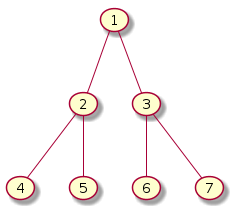
\includegraphics[scale=0.5]{ressources/images/Tree.png}
                \caption{A tree}
                \label{Tree}
            \end{figure}
            \subsubsection{Forest}
            A \textbf{forest} is a graph with no cycle\\
            \begin{figure}[h]
                \centering
                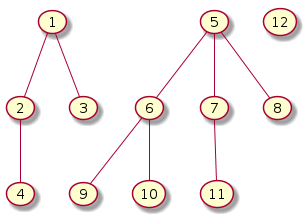
\includegraphics[scale=0.5]{ressources/images/Forest.png}
                \caption{A forest}
                \label{Forest}
            \end{figure}
        \subsubsection{Equivalence on trees}
            The following are equivalent: \\
            \begin{enumerate}
                \item $T$ is a tree
                \item $T$ is loopless and for $v, w \in V(T)$, $T$ has a UNIQUE path from $v$ to $w$
                \item $T$ is connected and $T$\\$e$ is disconnected from all $e\in E(T)$
                \item $T$ has no cycle and $T + xy$ (adding a new edge $xy$ to $T$) has a cycle for any $x, y \in V(G)$
            \end{enumerate}
        \subsubsection{Lemma}
            If $T$ is a tree with at least 1 vertex, then $|E(T)|=|V(T)|-1$
        \subsubsection{Proof}
            Induction on $|E(T)|$\\
            If $E(T)=\emptyset, \Rightarrow|V(T)|=1\Rightarrow 1-1=0$\\
            Now let $e\in E(T)$\\
            $T\backslash e$ has exactly 2 components $T_1, T_2$\\
            $|E(T_1)|=|V(T_1)|-1$\\
            $|E(T_2)|=|V(T_2)|-1$\\
            \begin{figure}[h]
                \centering
                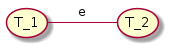
\includegraphics[scale=0.5]{ressources/images/BipartiteGraph2.png}
                \caption{A bipartite graph (With its 2 parts)}
                \label{Bipartite graph}
            \end{figure}
        \subsubsection{Corrolary}
            If $T$ is a tree with at least 2 vertices, then $T$ has a leaf
    \subsection{Bipartite graphs}
        $G$ is a \textbf{bipartite} graph if $G$ has a \textbf{bipartition} $(A, B)$ such that $A\cup B=V(G), A\cap B=\emptyset$and evey edge as 1 end on $A$, and another end on $B$
        \begin{figure}[h]
            \centering
            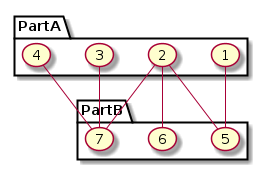
\includegraphics[scale=0.5]{ressources/images/BipartiteGraph.png}
            \caption{A bipartite graph (With its 2 parts)}
            \label{Bipartite graph}
        \end{figure}
    \subsection{Bipartite $\Leftrightarrow$ no odd cycle}
        \subsubsection{Definition}
            $G$ is bipartite $\Leftrightarrow G$ has no odd cycle
        \subsubsection{Proof}
            \begin{itemize}
                \item $\Rightarrow$: trivial
                \item $\Leftarrow$: Induction on $|E(G)|$\\
                    If $|E(G)|=0$, trivial\\
                    Let $e\in E(G)$\\
                    $G\backslash e$ has no odd cycle $\Rightarrow$ $G\ e$ is bipartite\\
                    $G\backslash e$ has a bipartition ($A, B$)\\
                    We may assume both ends are in $A$\\
                    If$G\backslash e$ has a path $P$ from $x$ to $y$, length of $P$ is even.\\
                    $P+e:=\text{odd cycle}$
            \end{itemize}
